\chapter{補間}
    \section{IDTFT を用いた有限長信号の補間}
        \subsection{動機}
            有限長の離散時間信号(例えば係数畳み込み型 FIR フィルタ係数)が与えられたとき、その信号を連続時間信号に拡張して、任意の時刻での値を求めたいときがある。
            例えば FIR フィルタのインパルス応答が離散時間信号として既知であるとき、非整数の時刻に於ける合理的な値を考えたい(これはアップ・サンプリングの為の poly-phase フィルタの係数を計算する方法の一つである)。
        \subsection{方法}
            \label{IDTFT を用いた有限長信号の補間の方法}
            台有界な離散時間信号 $\xd:\integers\to\complexNumbers$ の DTFT を $\Xd:\realNumbers\to\complexNumbers$ とする。
            但し引数は正規化角周波数である。
            連続時間信号 $\hat{x}:\realNumbers\to\realNumbers$ を次式で定義する。
            \[ \hat{x}(t)\coloneq\left.\IDTFT{\Xd}(n)\right|_{n\to t} = \frac{1}{2\pi}\integrate{-\pi}{\pi}{\Xd(\Omega)\exp\parens*{i\Omega t}}{}{\Omega} \]
            殆ど自明なことだが、$\hat{x}$ は全ての離散時刻に於いて $\xd$ と一致する連続関数である。
            \par
            例えば $\xd$ が既知であって、それをある時間 $d\in(0,1)$ だけ仮想的に遅らせた(サンプリング時刻が仮想的に $d$ だけ早まった)離散時間信号は $n\in\integers\mapsto\hat{x}(n-d)$ である。
            これも殆ど自明なことだが、この信号の DTFT のエネルギー・スペクトラム密度は $\xd$ のそれと等しい。
        \subsection{数値例}
            $N=33,\;\alpha=0.4$ とし、有限長の離散時間信号 $h:\integers\to\realNumbers$ を次式で定義する。
            これは視覚的な解り易さから \cite{learn_sp_from_basic} 式 (8.41) から流用したものである。
            \[
                h(n) = \begin{cases}
                    \alpha & (n=(N-1)/2) \\
                    \alpha\sinc{\parens*{(N-1)/2-\pi}\alpha\pi} & (n\in\{0,1,2,\dots,N-1\}\setminus\{(N-1)/2\}) \\
                    0 & (\text{otherwise})
                \end{cases}
            \]
            次の図は $h$ とその DTFT である。
            \begin{figure}[H]
                \centering
                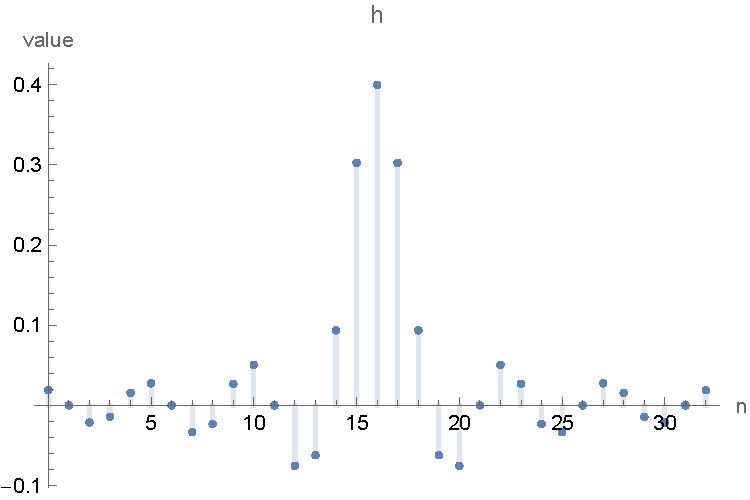
\includegraphics[keepaspectratio, scale=0.7]
                {\currfiledir/calc/Interpolation_with_DTFT_and_IDTFT/h.pdf}
                \caption{$h$}
            \end{figure}
            \begin{figure}[H]
                \centering
                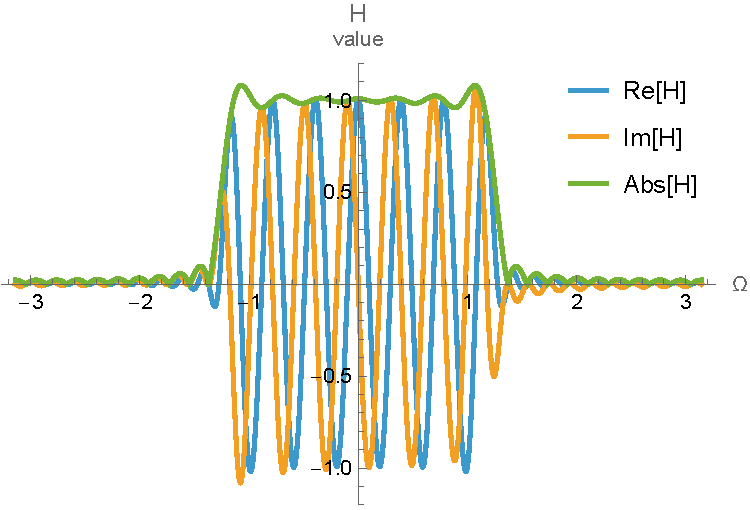
\includegraphics[keepaspectratio, scale=0.7]
                {\currfiledir/calc/Interpolation_with_DTFT_and_IDTFT/DTFT_of_h.pdf}
                \caption{$h$ の DTFT。横軸は正規化角周波数}
            \end{figure}
            これを前小節の方法で実時間信号に拡張したものを $\tilde{h}$ とする。
            次の図は $h$ と $\tilde{h}$ を重ねて描いたものである。
            \begin{figure}[H]
                \centering
                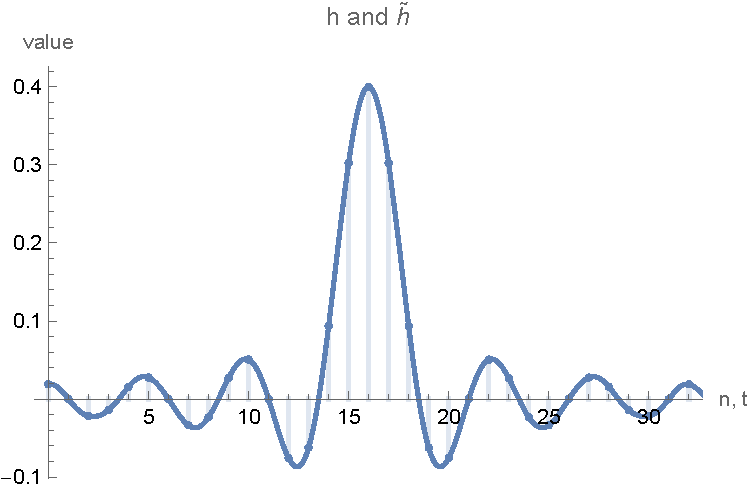
\includegraphics[keepaspectratio, scale=0.7]
                {\currfiledir/calc/Interpolation_with_DTFT_and_IDTFT/h_and_h_tilde.pdf}
                \caption{$h$ と $\tilde{h}$}
            \end{figure}
            新たな離散時間信号 $h^\dagger:(d,n)\in\realNumbers\times\integers\mapsto\tilde{h}(n-d)$ を定義する。
            $h^\dagger$ は $h$ を仮想的に $d$ だけ遅らせたものである。
            \begin{figure}[H]
                \centering
                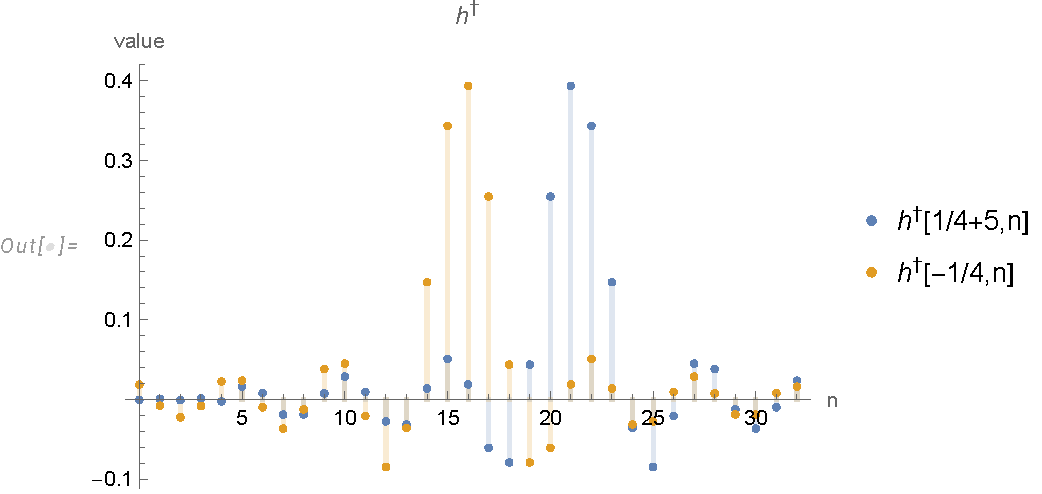
\includegraphics[keepaspectratio, scale=0.7]
                {\currfiledir/calc/Interpolation_with_DTFT_and_IDTFT/h_and_h_dag.pdf}
                \caption{$h^\dagger,\quad d=-0.25,\;0.75$}
            \end{figure}
            この数値例を計算した Mathematica notebook が下記のファイル名で保存されている。
            Git リポジトリ内でファイル名検索すれば発見できるであろう。
            notebook 中では前記 $N$ が \inlineCode{N_tp} となっている。\newline
            \href{\currfiledir/calc/Interpolation_with_DTFT_and_IDTFT/Interpolation_with_DTFT_and_IDTFT.nb}{Interpolation\_with\_DTFT\_and\_IDTFT.nb}\newline
        \subsection{等間隔補間信号の周波数スペクトラム}
            \newcommand{\Xdn}{X_\text{d,n}}
            \newcommand{\Ydn}{Y_\text{d,n}}
            \ref{IDTFT を用いた有限長信号の補間の方法} の方法で等間隔に補間され $L\;(\in\naturalNumbers,L\geq 2)$ 倍のサンプル周波数を持つ新たな信号の周波数スペクトラムの性質を述べる。
            \begin{shadebox}
                $L$ を 2 以上の自然数とする。
                サンプル周期 $\Ts>0$ の離散時間信号 $\xd:\integers\to\complexNumbers$ を \ref{IDTFT を用いた有限長信号の補間の方法} の方法で等間隔に補間し、サンプル周期 $\Ts/L$ となった離散時間信号を $\yd$ とする。
                但し $\xd,\;\yd$ 両方のサンプリング時刻が 0 を含むものとする。
                $\Xd,\;\Yd$ を $\xd,\;\yd$ の DTFT とする。
                次式が成り立つ。
                \[ \Yd(\omega) = L\sum_{n=-\infty}^\infty \Xd\parens*{\omega-n\frac{2\pi L}{\Ts}}\uBox\parens*{\frac{\Ts}{2\pi}\parens*{\omega-\frac{2\pi L}{\Ts}n}} \tag{1} \]
                元のサンプル周期に於ける第 1 Nyquist 領域の外側で $\Xd$ を 0 としたものが、 $\Ts/(2\pi L)$ 周期拡張されている。
                \par
                $\Xdn,\;\Ydn$ を $\xd,\;\yd$ の DTFT であって引数が正規化角周波数であるものとする(前者と後者の正規化角周波数はスケールが異なる。それぞれ $\omega\Ts,\;\omega\Ts/L$)。
                これを用いて式 (1) を書き直すと次式である。
                \[ \Ydn(\Omega) = L\sum_{n=-\infty}^\infty \Xdn\parens*{L(\Omega-2\pi n)}\uBox\parens*{\frac{L}{2\pi}\parens*{\Omega-2\pi n}} \tag{2} \]
                元のサンプル周期に於ける第 1 Nyquist 領域の外側で $\Xdn$ を 0 とした後に角周波数軸方向に $1/L$ 倍に縮めたものが $2\pi$ 周期拡張されている。
            \end{shadebox}
            \begin{proof}
                \begin{align*}
                    \yd(n) &= \left.\xd(n)\right|_{n\to n/L} = \frac{\Ts}{2\pi}\integrate{\pi/\Ts}{-\pi/\Ts}{\Xd(\omega)\exp(i\omega n\Ts/L)}{}{\omega} \\
                    \Yd(\omega) &= \sum_{n=-\infty}^\infty \yd(n)\exp(-i\omega n\Ts/L) \tag{3} \\
                    &= \sum_{n=-\infty}^\infty \frac{\Ts}{2\pi}\integrate{\pi/\Ts}{-\pi/\Ts}{\Xd(\tilde{\omega})\exp(i\tilde{\omega} n\Ts/L)}{}{\tilde{\omega}}\exp(-i\omega n\Ts/L) \\
                    &= \frac{\Ts}{2\pi}\integrate{\pi/\Ts}{-\pi/\Ts}{\Xd(\tilde{\omega})\sum_{n=-\infty}^\infty\exp(i(\tilde{\omega}-\omega)n\Ts/L)}{}{\tilde{\omega}} \\
                    &= \frac{\Ts}{2\pi}\integrate{\pi/\Ts}{-\pi/\Ts}{\Xd(\tilde{\omega})\frac{2\pi L}{\Ts}\sum_{n=-\infty}^\infty\delta(\tilde{\omega}-\omega-2\pi Ln/\Ts)}{}{\tilde{\omega}} \quad (\text{\ref{定数関数1のDTFT}} を用いた) \\
                    &= L\sum_{n=-\infty}^\infty\integrate{\pi/\Ts}{-\pi/\Ts}{\Xd(\tilde{\omega})\delta(\tilde{\omega}-\omega-2\pi Ln/\Ts)}{}{\tilde{\omega}}
                \end{align*}
                この式の評価には注意を要する。
                式 (3) より $\Yd$ が $2\pi L/\Ts$ 周期関数であることが解るから、区間 $[-\pi L/\Ts,\pi L/\Ts]$ に於ける式を構築した後に $2\pi L/\Ts$ 周期拡張すればよい。
                \par
                まず $\omega\in[-\pi L/\Ts,\pi L/\Ts]\setminus[-\pi/\Ts,\pi/\Ts]$ のとき、$n$ がどうであっても $\omega+2\pi Ln/\Ts$ は $[-\pi/\Ts,\pi/\Ts]$ に属さないから $\Yd(\omega)=0$ である。
                次に $\omega\in[-\pi/\Ts,\pi/\Ts]$ のとき、$\omega+2\pi Ln/\Ts$ は $n=0$ のとき、かつそのときに限り $[-\pi/\Ts,\pi/\Ts]$ に属すから $\Yd(\omega)=\Xd(\omega)$ である。
                以上 2 つから、区間 $[-\pi L/\Ts,\pi L/\Ts]$ に於いては $\Yd(\omega) = \Xd(\omega)\uBox(\omega\Ts/(2\pi))$ である。
                これを $2\pi L/\Ts$ 周期拡張すれば式 (1) が得られる。
                \par
                式 (1) に於いて $\omega$ を $\Omega/\Ts$ で書き換え、関係式 $\Xd(\Omega/\Ts) = X(\Omega)$ を用いると式 (2) が得られる。
            \end{proof}
            \subsubsection{数値例}